%************************************************
\chapter{To make a sub distribution board}
%************************************************
\begin{flushright}
September 1, 2012
\end{flushright}
\section{Aim}
To make a sub-distribution board for controlling a Lamp, a Fan (via a Ceiling Rose) and a Power Socket, using three separate switches.

\section{Theory}
	This sub-distribution board is designed to control one lamp, one power socket and a fan. The switches are connected in parallel. The neutral and earth (ground) connections are common.
	\subsection {Tools}
		\begin{enumerate}
			\item Pliers
			\item Screwdriver
			\item Electrical Line Tester
		\end{enumerate}
	\subsection {Material}
		\begin{enumerate}
			\item Single way switch
			\item Lamp
			\item Lamp Holder
			\item Bakelite Sheet
			\item Wires
			\item Screws
			\item Nut Bolts
			\item Ceiling Hose
			\item Terminals
		\end{enumerate}
\section{Procedure}
	\begin{enumerate}
		\item Took a suitable Bakelite sheet and attached the following using screws \& nut-bolts
			\begin{enumerate}
				\item Power Connectors
				\item Switch
			\end{enumerate} 
		\item Connected the circuit according to the circuit diagram as given in \autoref{E3_fig1}, keeping the following in mind
		\begin{figure}[bth]
			\begin{center}
				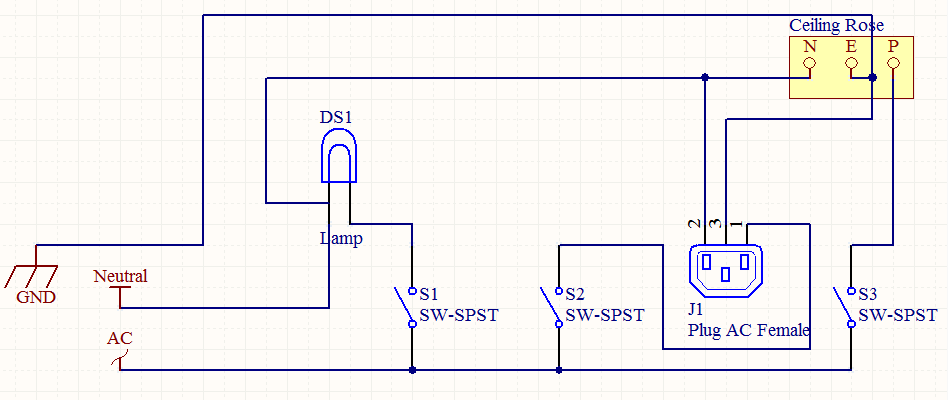
\includegraphics[width=1.2\linewidth]{gfx/circuit3}
			\end{center}
		\caption[Redistribution Board]{Redistribution Board}\label{E3_fig1}
		\end{figure}

			\begin{enumerate}
				\item \emph{Red Wires} are used for the phase connections.
				\item \emph{Black Wires} are used for the neutral connections.
				\item Colours other than Red, Black and Green can be used for the connecting wires.
			\end{enumerate}	
		\item Attached the remaining components using screws \& nut-bolts.
	\end{enumerate}
\section{Precaution}
	\begin{enumerate}
		\item Connections should be tight, viz. shouldn't come out when pulled.
		\item Wires shouldn't be sticking out of the connections without insulation.
		\item Wires should be of appropriate length.
		\item Colours of the wires should be chosen in accordance with their type.
	\end{enumerate}	
\section{Acknowledgements}
I thank Mr. Jatinder Singh for his guidance during the experiment.